\section{Results}
\label{sec:results}

In order to report results in a readable format, we discuss each model in a separate subsection by also providing a table summarizing the results. In the leftmost part, each table reports the list of variables included in the full-factorial version of each model. In the central part, model-simplification procedure (\emph{Removal order}), chi-square goodness-of-fit test (\emph{Chi-square}) and its results (\emph{p}) are reported. The rightmost part shows the effects of the variables included in the final model.

\begin{table}[t!]
\centering
\small
\begin{tabular}{|l|l|l|l|l|l|l|}
\hline
Parameter                    & Chi-square & p      & Removal order & Estimate & z-value & p      \\ \hline
(Intercept)                  & --       & --     & Not removed   & -0.8362  & -0.741  & 0.4587 \\
MCsim & --       & --     & Not removed   & -6.4337  & -2.361  & 0.0182 \\
HCsim     & --       & --     & Not removed   & -5.5904  & -2.102  & 0.0355 \\
Density         & --       & --     & Not removed   & 7.6332   & 1.916   & 0.0553 \\
PMI & --       & --     & Not removed   & 0.0878   & 1.885   & 0.0594 \\
MHsim     & 2.5275   & 0.1119 & 6             &          &         &        \\
Head freq               & 0.7637   & 0.3822 & 5             &          &         &        \\
Mod freq           & 0.4882   & 0.4847 & 4             &          &         &        \\
Comp length              & 0.8206   & 0.365  & 3             &          &         &        \\
Comp freq           & 0.0745   & 0.7848 & 2             &          &         &        \\
Entropy                      & 0.005    & 0.9433 & 1             &          &         &        \\ \hline
\end{tabular}
\caption{Results of the logit model opposing ATT (1) to SUB (0).}
\label{tab:resattsub}
\end{table}

\subsection{ATT vs SUB}

The first model, testing ATT (\emph{halfprice}) against SUB (\emph{bus-stop}) compounds, reliably distinguishes the two classes on semantic bases. As shown in Table~\ref{tab:resattsub}, SUB is predicted against ATT by the higher semantic similarity between the compound and either the modifier (\emph{p}=.0182) or the head (\emph{p}=.0355). That is, the meaning of SUB compounds such as \emph{bus-stop} is found to be more strongly determined by the individual meanings of its constituents compared to ATT compounds like \emph{halfprice}, since both the modifier and the head contribute to the overall meaning to a greater extent than either constituents of ATT compounds do. Therefore, the higher the similarity between the compound and either constituents, the higher the probability to have a SUB rather than an ATT compound.

It should be noted that frequency measures, entropy, compound length and the similarity between the two constituents were progressively removed from the model. That is, their effects do not contribute to predict one class over the other. The remaining variables, namely PMI and neighborhood density, are instead included in the final model, even though their effect is only partially reliable (\emph{p}>.05). Both these measures, anyway, indicate that higher values of both PMI and density are more likely to predict ATT rather than SUB compounds.



\subsection{ATT vs CRD}

The second model tests ATT (\emph{halfprice}) against CRD (\emph{comedy-drama}) compounds. As reported in Table~\ref{tab:resattcrd}, our model reliably distinguishes between the two classes on the basis of a single, highly significant semantic predictor, namely the semantic similarity between the compound constituents (\emph{p}=.0002). In particular, the higher the similarity between the modifier and the head of a compound, the higher the probability of having a CRD, rather than an ATT compound. All other variables have been progressively removed from the final model since none of them significantly contribute to the overall goodness fit.

\begin{table}[t!]
\centering
\small
\begin{tabular}{|l|l|l|l|l|l|l|}
\hline
Parameter   & Chi-square & p      & Removal order & Estimate & z-value & p      \\ \hline
(Intercept) & --       & --     & Not removed   & 5.667    & 4.094   & 0.0001 \\
MHsim       & --       & --     & Not removed   & -18.182  & -3.667  & 0.0002 \\
Comp length & 2.0539   & 0.1518 & 9             &          &         &        \\
Comp freq   & 1.2866   & 0.2567 & 8             &          &         &        \\
Head freq   & 0.77     & 0.3802 & 7             &          &         &        \\
HCsim       & 0.8033   & 0.3701 & 6             &          &         &        \\
MCsim       & 0.5967   & 0.4398 & 5             &          &         &        \\
Mod freq    & 0.7654   & 0.3816 & 4             &          &         &        \\
PMI         & 0.5182   & 0.4716 & 3             &          &         &        \\
Entropy     & 0.1344   & 0.7139 & 2             &          &         &        \\
Density     & 0.0346   & 0.8524 & 1             &          &         &        \\ \hline
\end{tabular}
\caption{Results of the logit model opposing ATT (1) to CRD (0).}
\label{tab:resattcrd}
\end{table}

\subsection{CRD vs SUB}

\begin{table}[b!]
\centering
\small
\begin{tabular}{|l|l|l|l|l|l|l|}
\hline
Parameter   & Chi-square & p      & Removal order & Estimate & z-value & p      \\ \hline
(Intercept) & --       & --     & Not removed   & -0.0843  & -0.037  & 0.9707 \\
MHsim       & --       & --     & Not removed   & 36.3465  & 3.03    & 0.0024 \\
HCsim       & --       & --     & Not removed   & -25.2847 & -2.44   & 0.0146 \\
Comp length & --       & --     & Not removed   & -0.5323  & -1.996  & 0.0459 \\
PMI         & 0.3016   & 0.5828 & 7             &          &         &        \\
Comp freq   & 0.3286   & 0.5665 & 6             &          &         &        \\
MCsim       & 0.2825   & 0.595  & 5             &          &         &        \\
Density     & 0.1055   & 0.7453 & 4             &          &         &        \\
Entropy     & 0.2244   & 0.6357 & 3             &          &         &        \\
Mod freq    & 0.1236   & 0.7251 & 2             &          &         &        \\
Head freq   & 0.0084   & 0.9267 & 1             &          &         &        \\ \hline
\end{tabular}
\caption{Results of the logit model opposing CRD (1) to SUB (0).}
\label{tab:reascrdsub}
\end{table}

The third model opposes CRD (\emph{comedy-drama}) to SUB (\emph{bus-stop}) compounds. Also in this case, the model reliably distinguishes between one class and the other on semantic bases. In particular, CRD is predicted over SUB by the degree of semantic similarity between the two constituents (\emph{p}=.0024). The greater the similarity between the modifier and the head of a compound, the higher the probability of having a CRD rather than a SUB compound. Also, SUB is predicted over CRD by the degree of similarity between the compound and its head (\emph{p}=.0146). That is, the head constituent contributes more to the overall meaning of SUB compounds (e.g., \emph{stop} in \emph{bus-stop}) than CRD compounds (e.g., \emph{drama} in \emph{comedy-drama}).

In addition to these semantic variables, compound length turns out to be also predictive of one class over the other. As reported in Table~\ref{tab:reascrdsub}, in fact, its effect is reliable (\emph{p}=.0459) and it indicates that longer compounds are more likely to be SUB than CRD. All other parameters were instead progressively removed.

\subsection{Overall results}

\begin{figure}[t!]
\begin{center}
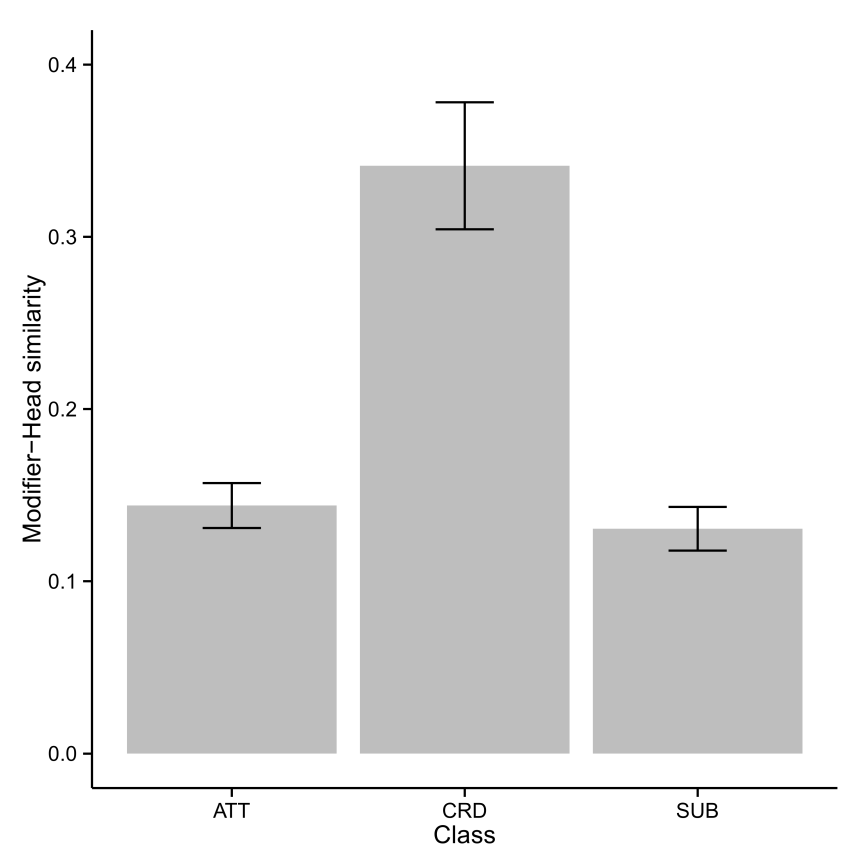
\includegraphics[scale=0.9]{figures/barplot1.png}
\caption{Similarity between modifier and head is predictive of CRD over both ATT and SUB.}\label{fig:bar1}
\end{center}
\end{figure}


Taken together, these results indicate that the degree of semantic similarity between the compound constituents (i.e. the modifier and the head) is a highly reliable predictor of CRD against both other classes. As shown in the barplot in Figure~\ref{fig:bar1}, the higher the similarity between the constituents, the more a compound is likely to be CRD rather than either ATT (\emph{p}=.0002) or SUB (\emph{p}=.0024). Moreover, the semantic similarity between the compound and its head is a predictive measure of SUB over both other types, as shown in Figure~\ref{fig:bar2}. That is, the more the head contributes to the meaning of the overall compound, the more the compound is likely to be SUB rather than either ATT (\emph{p}=.0355) or CRD (\emph{p}=.0146).

\begin{figure}[t!]
\begin{center}
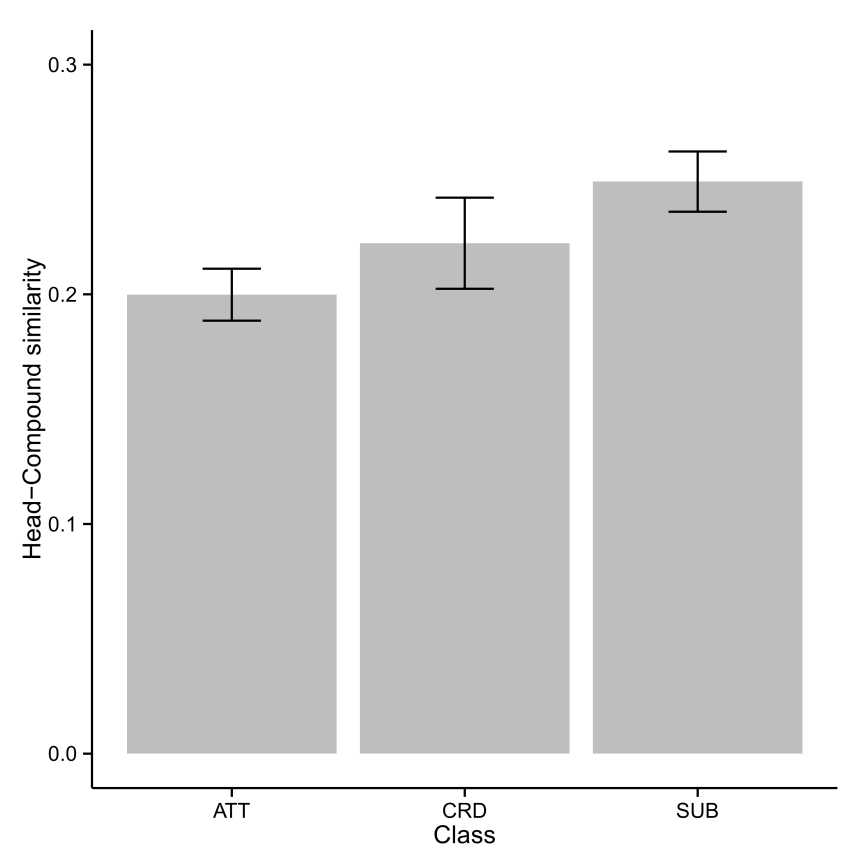
\includegraphics[scale=0.9]{figures/barplot2.png}
\caption{Similarity between the compound and its head is predictive of SUB over both ATT and CRD.}\label{fig:bar2}
\end{center}
\end{figure}


In order to evaluate the predictive power of each model, we further computed the accuracy with which the items under investigation were correctly assigned to the correct classes. First, we obtained the classes predicted by each logit model. Second, we computed the accuracy of each model by dividing the number of correctly predicted items by the total number of items included in the final model. As a comparison, for each model we also computed the accuracy of a majority baseline obtained by simply dividing the number of cases of the majority class by the total number of cases involved.  As reported in Table~\ref{tab:qualres}, the best predictive model turned out to be the one opposing CRD vs SUB (.90 accuracy) followed by ATT vs CRD (.85) and ATT vs SUB (.61). These numbers were in line with the pattern of accuracies obtained by the majority baseline, which is sensible to the low number of CRD cases and therefore outputs higher scores for comparisons involving this class. Though our models always outperformed the baselines, the increase was sensibly lower in ATT vs SUB (+3\%) compared to both CRD vs SUB (+9\%) and ATT vs CRD (+10\%). The limited number of items do not allow us to make any statistically reliable claim on the performance of the classifier. However, our focus is on testing whether the membership in a compound class is affected by a set of theoretically-relevant variables rather than proposing an effective classification algorithm. In this light, our results provided evidence for the effectiveness of these models. At the same time, they suggested that experimenting with more data would be desirable to further validate their power.



Besides accuracies, Table~\ref{tab:qualres} reports some correctly-predicted and missed cases for each of the models.





\begin{table}[t!]
\centering
\begin{tabular}{|l|l|l|l|}
\hline
Model   & Accuracy (baseline) & Predicted cases                                                                                                                   & Missed cases                                                                                                                 \\ \hline
ATT-SUB & 0.61 (0.58)     & \textit{\begin{tabular}[c]{@{}l@{}}able-bodied (ATT)\\ long-awaited (ATT)\\ schoolteacher (SUB)\\ racingclub (SUB)\end{tabular}}  & \textit{\begin{tabular}[c]{@{}l@{}}commonroom (ATT)\\ ironcurtain (ATT)\\ underbody (SUB)\\ apronstring (SUB)\end{tabular}}  \\ \hline
ATT-CRD & 0.85 (0.75)    & \textit{\begin{tabular}[c]{@{}l@{}}best-equipped (ATT)\\ keyword (ATT)\\ father-daughter (CRD)\\ comedy-drama (CRD)\end{tabular}} & \textit{\begin{tabular}[c]{@{}l@{}}bodypolitic (ATT)\\ highschool (ATT)\\ typewrite (CRD)\\ subject-verb (CRD)\end{tabular}} \\ \hline
CRD-SUB & 0.90 (0.81)    & \textit{\begin{tabular}[c]{@{}l@{}}comedy-drama (CRD)\\ blue-black (CRD)\\ bus-stop (SUB)\\ cutthroat (SUB)\end{tabular}}         & \textit{\begin{tabular}[c]{@{}l@{}}schoolteacher (SUB)\\ sleepwalk (SUB)\\ typewrite (CRD)\\ subject-verb (CRD)\end{tabular}} \\ \hline
\end{tabular}
\caption{From left to right: overall accuracy of each model as compared to the accuracy of the majority baseline, correctly predicted cases, missed cases. In brackets we report the correct class.}
\label{tab:qualres}
\end{table}
